\chapter{System Level Analyis}%
\section{Original Lineup}%
\subsection{Overview}%

Here is the system requirements, it's a Macro-cell basestation 
reciever  with multi-standards , RF frequency Band from 400MHz 
to 8GHz  with RF Bandwidth of 400MHz , the reciever is a
direct conversion reciever with intended Baseband Bandwidth  of 
200MHz , but due to Digital pre-distortion bandwidth is increased
to 600MHz,here is the original Lineup specifications shown in Figure~\ref{fig:orignal_lineup} , 
Table~\ref{tab:original_specs} and Table~\ref{tab:original_ADC_specs}
for ADC.
\begin{figure}[htpb]
    \centering
    
\includegraphics[width=0.8\textwidth]{Lineup_original.eps}
    \caption{Original Lineup Block diagram}
    \label{fig:orignal_lineup}
\end{figure}
\begin{table}[htbp]
    \centering
    \label{tab:original_specs}
    \caption{Receiver Chain Block Specifications}
    % \textwidth forces the table to fit your exact page margins
    \begin{tabularx}{\textwidth}{l c c c X} 
        \toprule
        \textbf{Block} & \textbf{Gain} & \textbf{Noise Figure} & \textbf{OIP3} & \textbf{Other Specs} \\ 
        \midrule
        First LNA (External)  & 20 dB & 2 dB & 35 dBm & \\ 
        Second LNA (Internal) & 14 dB & 3 dB & 33 dBm & \\ 
        DSA                   & -3 dB & 3 dB & 33 dBm & Control range = 15 dB \\ 
        Mixer                 & -7 dB & 7 dB & 15 dBm & \\ 
        LPF                   & -2 dB & 2 dB & 34 dBm & 0.5\,dB-BW = 250\,MHz, \newline 3\,dB-BW = 600\,MHz \\ 
        \bottomrule
    \end{tabularx}
\end{table}

\begin{table}[htbp]
    \centering
    \label{tab:original_ADC_specs}
    \caption{ADC Specifications}
    % \textwidth forces the table to fit your exact page margins
    \begin{tabular}{l c c} 
        \toprule
        \textbf{Paramter} & \textbf{Value} & \textbf{Unit} \\
        \midrule
        Input referred full-scale & -10 & dBm \\
        Resolution & 10 & bits \\ 
        Sampling frequency & 2.4 & GHz \\
        NSD & -149 & dBFS/Hz \\
        \bottomrule
    \end{tabular}
\end{table}

It's clear from the specifications for the RF chain that it's 
requires very high linearity, this is mainly due to the large 
in-band blocker, our Analyis will focus on only one CW blocker
that has -15dBm power described in LTE standard \cite{3gpp_ts36104_blocking}.

\subsection{Cascade Analyis}%
At Maximum Gain : Noise figure = 2.05dB , IIP3 = -9.97dBm , 
Gain = 22dB.\\
This means sensitivity of this reciever (Assuming minimum 
accepted SNR = 0dB).
\begin{equation}
    P_{noise_{RF}} = -174 + NF  + 10*\log(BW_{RF})
    \label{eq:noise_RF}
\end{equation}
\begin{equation}
    P_{noise_{ADC}}  = -149 + 10*\log(BW_{BB}) - Gain_{RF}
    \label{eq:noise_ADC}
\end{equation}
from equations~\ref{eq:noise_RF} ,\ref{eq:noise_ADC} , then 
$P_{sense} = -83.85 dBm$.

At minimum Gain: Noise figure =2.54dB , IIP3 = -1.94dBm ,
Gain = 7dB.\\
since
$P_{ADC_{FS}} = -10 dBm$ and this is an OFDM system that requires
PAR = 10dB , then Maximum average power should be $P_{max} = -27 
dBm$ and the SDR at this power (under no blocking conditions) 
according to equation~\ref{eq:SDR}, $SDR = 50dB$ at max power.\\
\begin{equation}
    SDR = 2(IIP3-P_{in})
    \label{eq:SDR}
\end{equation}
In case of blocking (blocker power = -15dBm) at 100MHz away from
channel edge, then SDR relation is described by 
eq~\ref{eq:SDR_blocker}
\begin{equation}
    SDR  = 2 IIP_3 - P_{in} - P_{blocker}
    \label{eq:SDR_blocker}
\end{equation}
So SDR in this case : $SDR = 38dB$ , which is far less than 
no-blocking case, that's why the system requires this very high
linearity.

\section{Proposed Lineup}%
The biggest issue with the original lineup is
the very high OIP3 of LNA which is not possible to integrate,
to make it possible to integrate the LNA first thing is to 
reduce its OIP3, final block diagram of the system is shown
at Figure~\ref{fig:proposed_lineup}.

\begin{figure}[htpb]
    \centering
    
\includegraphics[width=0.8\textwidth]{Line_up_mod.pdf}
    \caption{Proposed Lineup}
    \label{fig:proposed_lineup}
\end{figure}
\subsection{Modifications to original lineup}%
Several modifications are made to get to the block diagram in 
Figure~\ref{fig:proposed_lineup}, first of them is addition 
of Baseband VGA.

\subsubsection{Baseband VGA}%
Since linearity is a big issue (under blocking) , we can't put 
large gain in the RF chain , so the remainng gain is added in
baseband after the filter which lead to the second modification
which is the filter in the baseband
\subsubsection{Modification to the filter}%
Since we added gain to the baseband we should filter the 
blocker not to degrade SDR ,also since the filter Required BW is
600MHz then the filter should have two modes; one for the main
signal and the other for DPD, the filter new specifications are
shown in Table~\ref{tab:filter_new_specs} 
\begin{table}[htpb]
    \centering
    \caption{Filter New specifications}
    \label{tab:filter_new_specs}
    \begin{tabular}{|c|c|}
        \hline
        Paramter& Value  \\ \hline
        Bandwidth (0.5dB) & 250MHz \\ \hline
        Rejection at (300MHz) & 30dB \\ \hline
        Bandwidth (Mode 2) & 600MHz \\ \hline
    \end{tabular}
\end{table}
\subsubsection{Modification to LNA}%
Now we can relax the linearity specifications to the LNA, also
it was found the given technology can achieve very low noise 
figures , so the new LNA specifications are shown in 
Table~\ref{tab:LNA_new_specs}
\begin{table}[htpb]
    \centering
    \caption{LNA new specifications}
    \label{tab:LNA_new_specs}
    \begin{tabular}{|c|c|}
        \hline
        Paramter & Value \\ \hline
        OIP3 & 25 dBm \\ \hline
        NF & 1 dB \\ \hline
        Gain & 22 dB \\ \hline
    \end{tabular}
\end{table}
\subsubsection{RF Amplifier}%
Since LNA gain is reduced in the RF chain alot of losses can 
degrade reciever noise figure , so an RF Amplifier is added 
to compensate for these losses.

\subsubsection{ADC power modification}%
Originally $P_{FS}$ for the ADC was -10dBm , which is suitable 
for sigma-delta ADCs with low Bandwidth , but since Bandwidth is 
increased to 600MHz (due to DPD) it was hard to impelement 
$\Sigma - \Delta $ ADC , so we switched to SAR ADC , but SAR 
ADC requires full swing, so $P_{FS}$ is changed to 14dBm instead
of -10dBm , also total chain gain is increased by 24dB.

\subsection{Final Linup specifications}%
Final Receiver chain specifications are shown in 
Table~\ref{tab:final_specs}.\\
At max gain : gain = 57dB , NF = 1.87 dB , IIP3 = -32 dBm.\\
At min gain : gain = 24dB , NF = 12.6 dB , IIP3 = -1.52 dBm.
\begin{table}[htbp]
    \centering
    \label{tab:final_specs}
    \caption{Final Receiver Chain Block Specifications}
    % \textwidth forces the table to fit your exact page margins
    \begin{tabularx}{\textwidth}{l c c c X} 
        \toprule
        \textbf{Block} & \textbf{Gain} & \textbf{Noise Figure} & \textbf{OIP3} & \textbf{Other Specs} \\ 
        \midrule
         LNA   & 22 dB & 1 dB & 25 dBm & \\ 
    First DSA & -3 dB & 3 dB & 25 dBm & Control range = 15 dB \\ 
        RF Amplifier & 8 dB & 2 dB & 25 dBm &  \\ 
    Second DSA & -2 dB & 2 dB & 25 dBm & Control range = 3 dB \\ 
        Mixer  & -7 dB & 7 dB & 16 dBm & \\ 
        LPF   & 0 dB & 12 dB & 16 dBm & 0.5\,dB-BW = 250\,MHz, \newline Rejection at 300\,MHz = 30dB  \\ 
        VGA & 39 dB & 3 dB & 25 dBm & Control range = 15 dB\\
        \bottomrule
    \end{tabularx}
\end{table}
\section{Receiver system simulation}%
\label{sec:Receiver system simulation}
\subsection{Simulation setup}%
For simulation setup , what we want to achieve is the SNR ,SDR and
SNDR , that is the required output of the simulation , 
for simulating SDR and non-linearites , power series (Memoriless-
Non-linear model ) is used equation~\ref{eq:lineup_power_series}
\begin{equation}
    V_{out} = \alpha_1 V_{in} + \alpha_2 V_{in}^2 + \alpha_3 
    V_{in}^3
    \label{eq:lineup_power_series}
\end{equation}
Also ADC noise is referred to the input according to equation~\ref{eq:noise_ADC}

This approach has some benifits like it takes the accounts for
not only IM3 but Gain compression and reciever desenstization
due to blockers , also it takes account for IM2s , so results 
from this simulation gives specification on small singal IP3 that
are approximatly valid for large signal (ignoring $\alpha_5$).

For Noise simulation Friis formula is used instead 
equation~\ref{eq:friis_formula_noise}
\begin{equation}
    F_{total} = F_1 + \frac{F_2 -1}{G_1} + \frac{F_2 -1 }{G_1 G_2}
    + \dots + \frac{F_n -1}{G_1 G_2 \dots G_{n-1}}
    \label{eq:friis_formula_noise}
\end{equation}
Signal paramters are shown in Table~\ref{tab:signal_paramters}, a
picture of Non-linearties output spectrum of the reciever it 
appears IM3 with signal itself , IM3 with blocker , IM2 and
DC component, Note that this spectrum is double sided we are 
only showing one side , also note that  Blackman Harris windowing
is used (it apears like 3dB less).

\begin{table}[htpb]
    \centering
    \caption{Signal Paramter Table}
    \label{tab:signal_paramters}
    \begin{tabular}{|c|c|}
        \hline
        Paramter &  Value \\ \hline 
        RF tone 1 & 1.17GHz \\ \hline
        RF tone 2 & 1.18GHz \\ \hline
        CW blocker Power & -15 dBm \\ \hline
        CW blocker frequency & 1.3GHz \\ \hline
        LO frequency & 1GHz \\ \hline
        Blocker appears at input power & $P_{sens}$ + 6dB
        \cite{3gpp_ts36104_blocking} \\ \hline
    \end{tabular}
\end{table}

\begin{figure}[htbp]
  \centering
  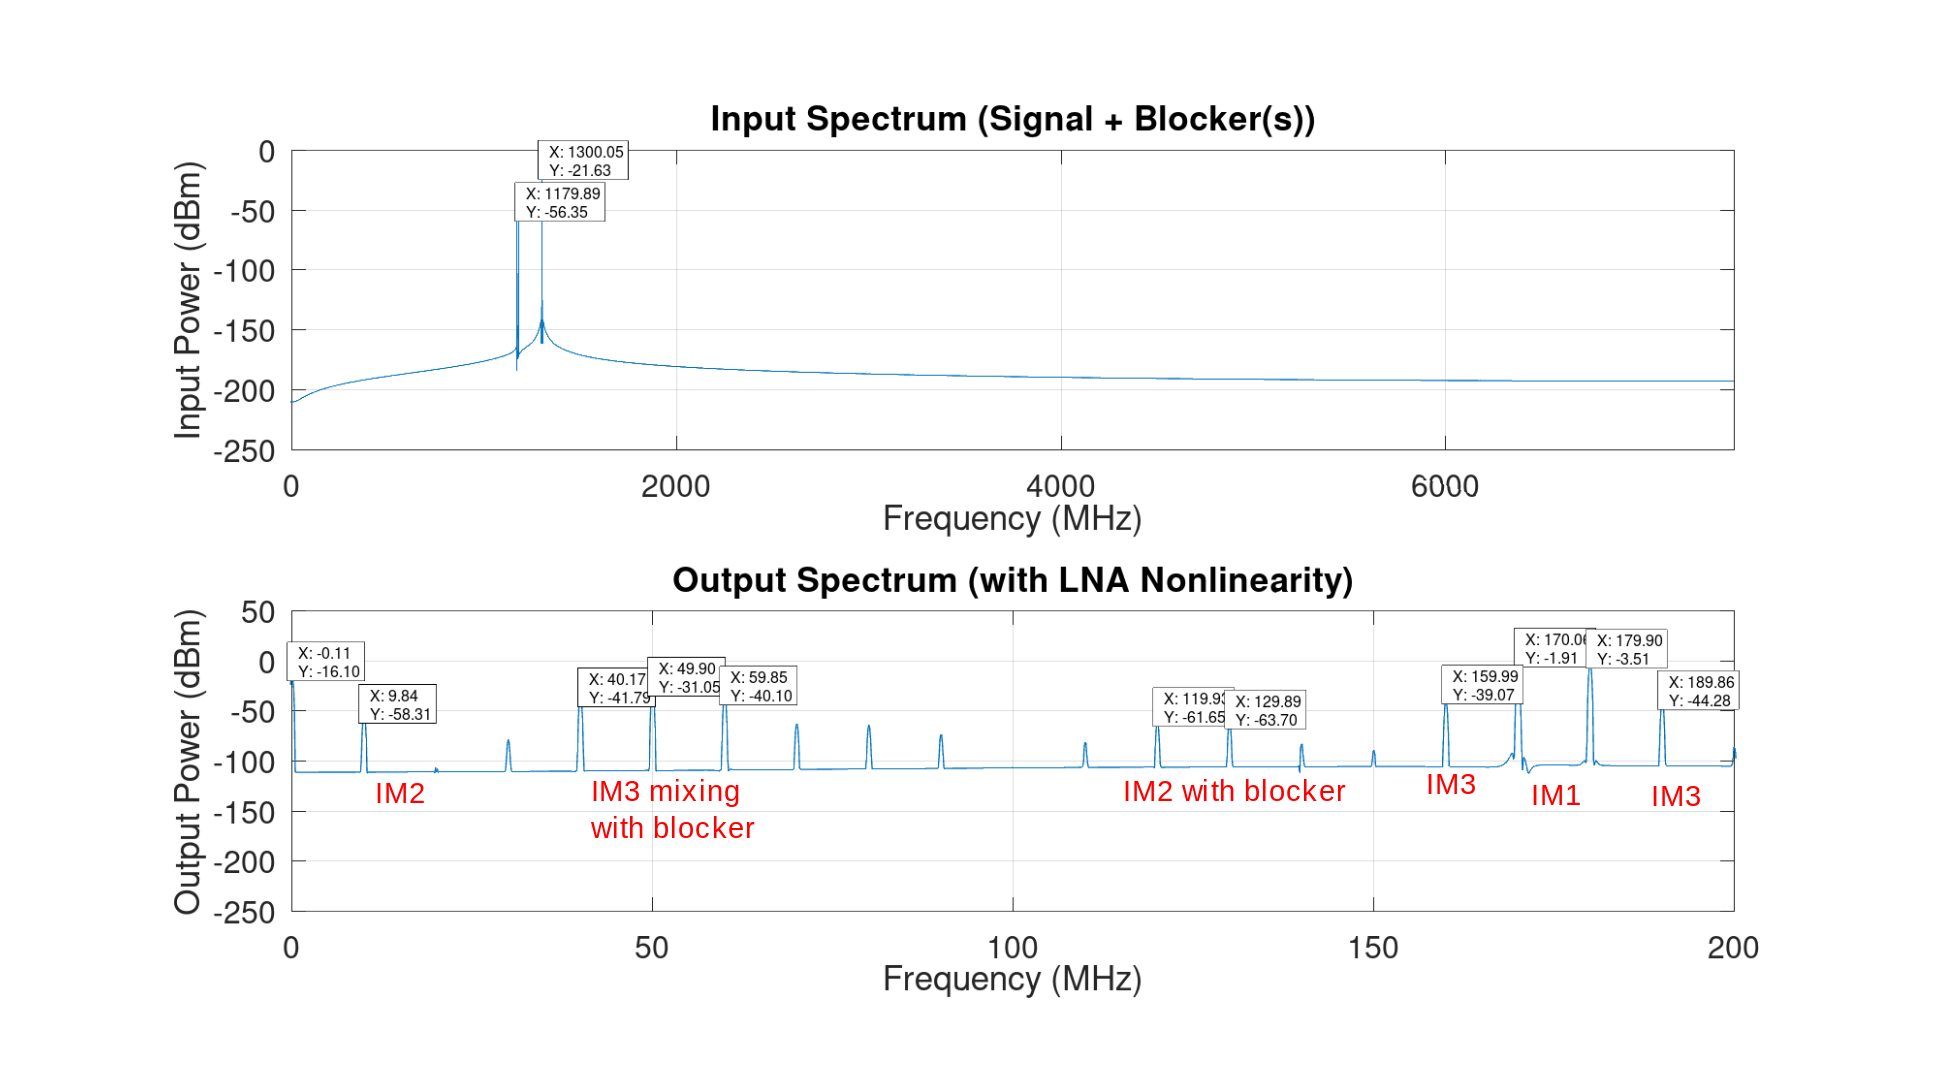
\includegraphics[width=1\linewidth]{images/Spectrum_Non_linearity.png}
  \caption{Output spectrum (Non-linearties) signal total
  power = -47dBm }
  \label{fig:Spectrum_Non_linearity.png}
\end{figure}

\subsection{Gain Policy}%
For the gain policy , two power detectors are placed , one at 
the output before ADC and the other afeter the mixer before LPF,
this power detector gives informations about the blocker existance.

\subsubsection{Attenuation Policy:}%
\label{ssub:Attenuation Policy:}
We need to calculate SDR degradation due to blocker this 
is described by equation~\ref{eq:SDR_blocker} so 
\[
    SDR_{due\ to\ blocker} = 2 IIP_{till \, LPF} - P_{in} -P_{blocker} -3  
\]
\[
    SDR = 2(OIP3_{till \, LPF} - G_{total} + G_{VGA} ) - P_{out} + G_{total} - P_{blocker} 
\]
\[
    SDR  = 2 OIP3_{till \, LPF} - (P_{out} + P_{mixer} + G_{LPF}) + G_{VGA} 
\]
    let  SDR  = X 
    \[
    P_{out} + P_{mixer}  \leq 2 OIP3_{till \, LPF} -X +G_{VGA} - G_{LPF}
\]
so final condition for Attenuation is given by
\begin{equation}
    P_{out} + P_{at\ mixer}  \geq 2 OIP3_{till \ LPF} + G_{VGA} - G_{LPF} - X
    \label{eq:DSA_atten_cond}
\end{equation}
Where X is some value chosen arbitrarly,when this condition
happens start Attenuation from first DSA, otherwise Attenuation 
starts with the baseband VGA when $P_{ADC}$ reaches maximum

\subsection{Simulation Results}%
\label{sub:Simulation Results}
\subsubsection{No blocking}%
\label{ssub:Under no blocking}
As shown in Figure~\ref{fig:VGA_policy_under_blocking.png} VGA starts the attenuation since there is no 
blocker and the condition at \ref{eq:DSA_atten_cond} is not satisfied.

\begin{figure}[!h]
  \centering
  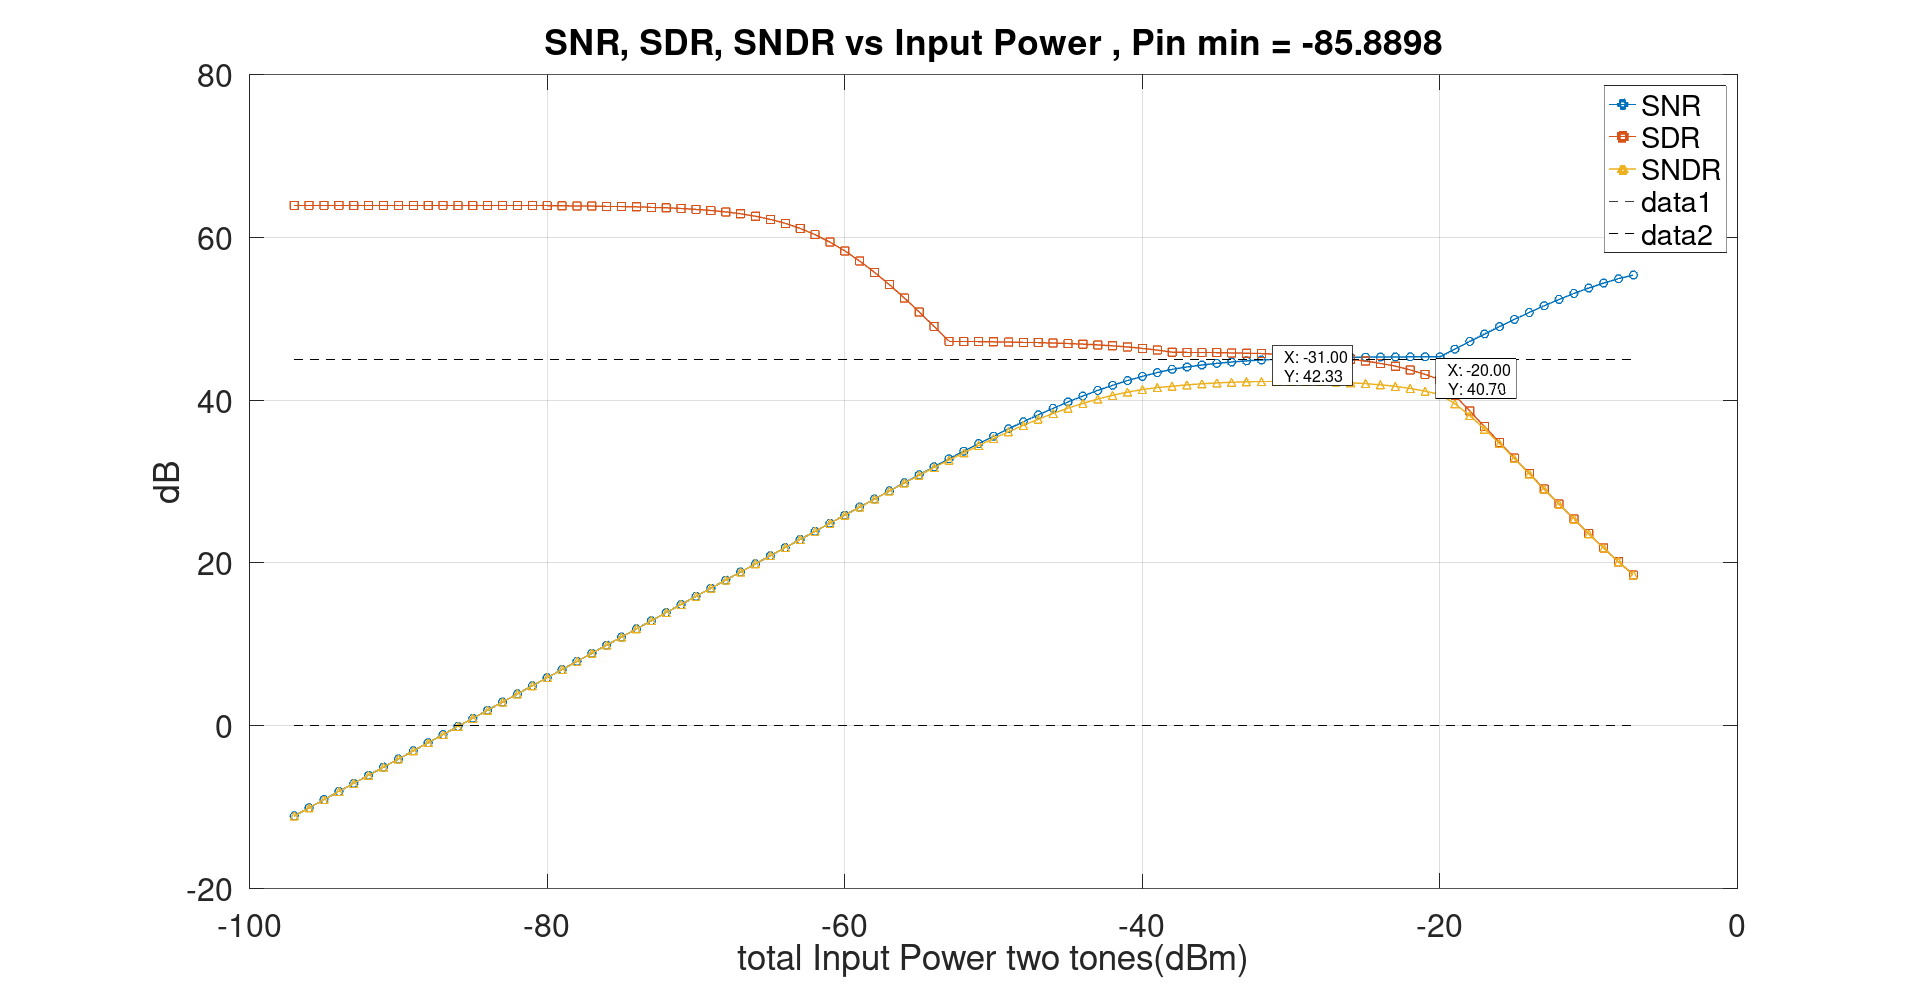
\includegraphics[width=1\linewidth]{images/SNDR_curve_No_blockers.png}
  \caption{SNDR curve no blockers}
  \label{fig:SNDR_curve_No_blockers.png}
\end{figure}

\begin{figure}[!h]
  \centering
  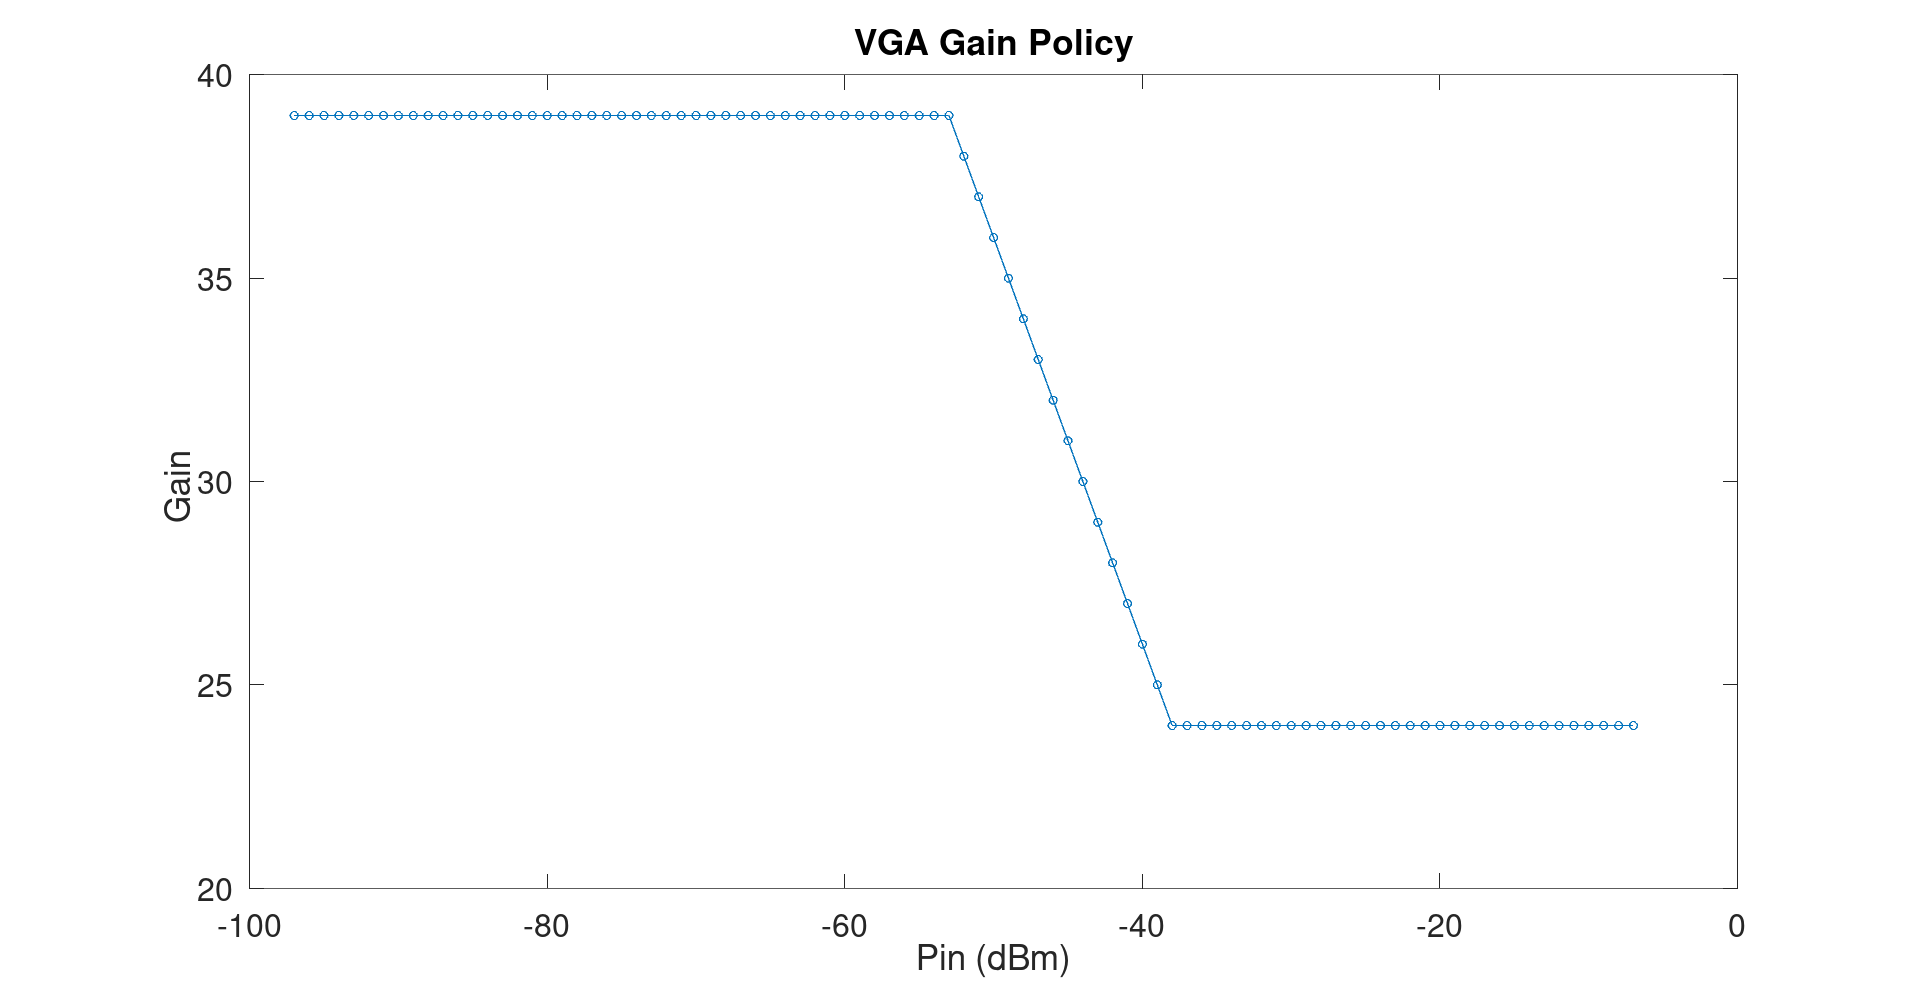
\includegraphics[width=1\linewidth]{images/VGA_no_policy_no_blockers.png}
  \caption{VGA Gain policy no blockers}
  \label{fig:VGA_no_policy_no_blockers.png}
\end{figure}
\begin{figure}[!h]
  \centering
  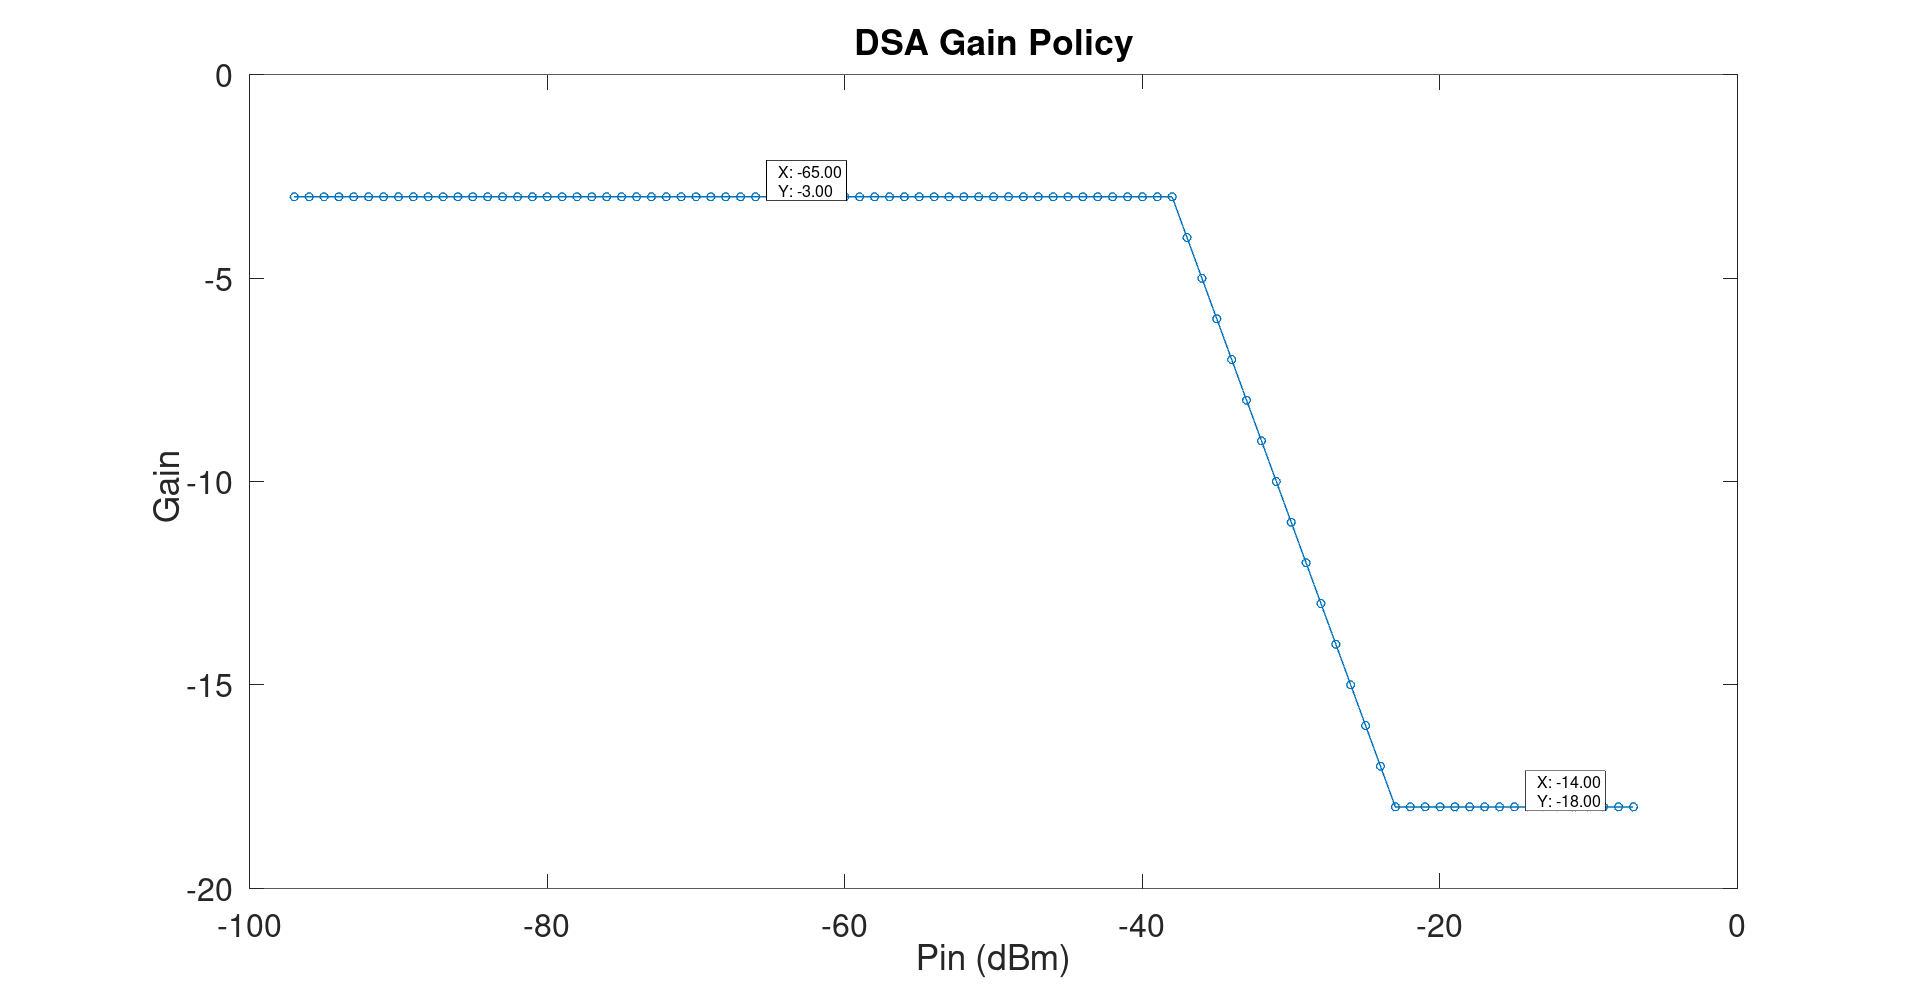
\includegraphics[width=1\linewidth]{images/DSA_1_gain_policy_no_blockers.png}
  \caption{DSA 1 Gain Policy no blockers}
  \label{fig:DSA_1_gain_policy_no_blockers.png}
\end{figure}

\begin{figure}[!h]
  \centering
  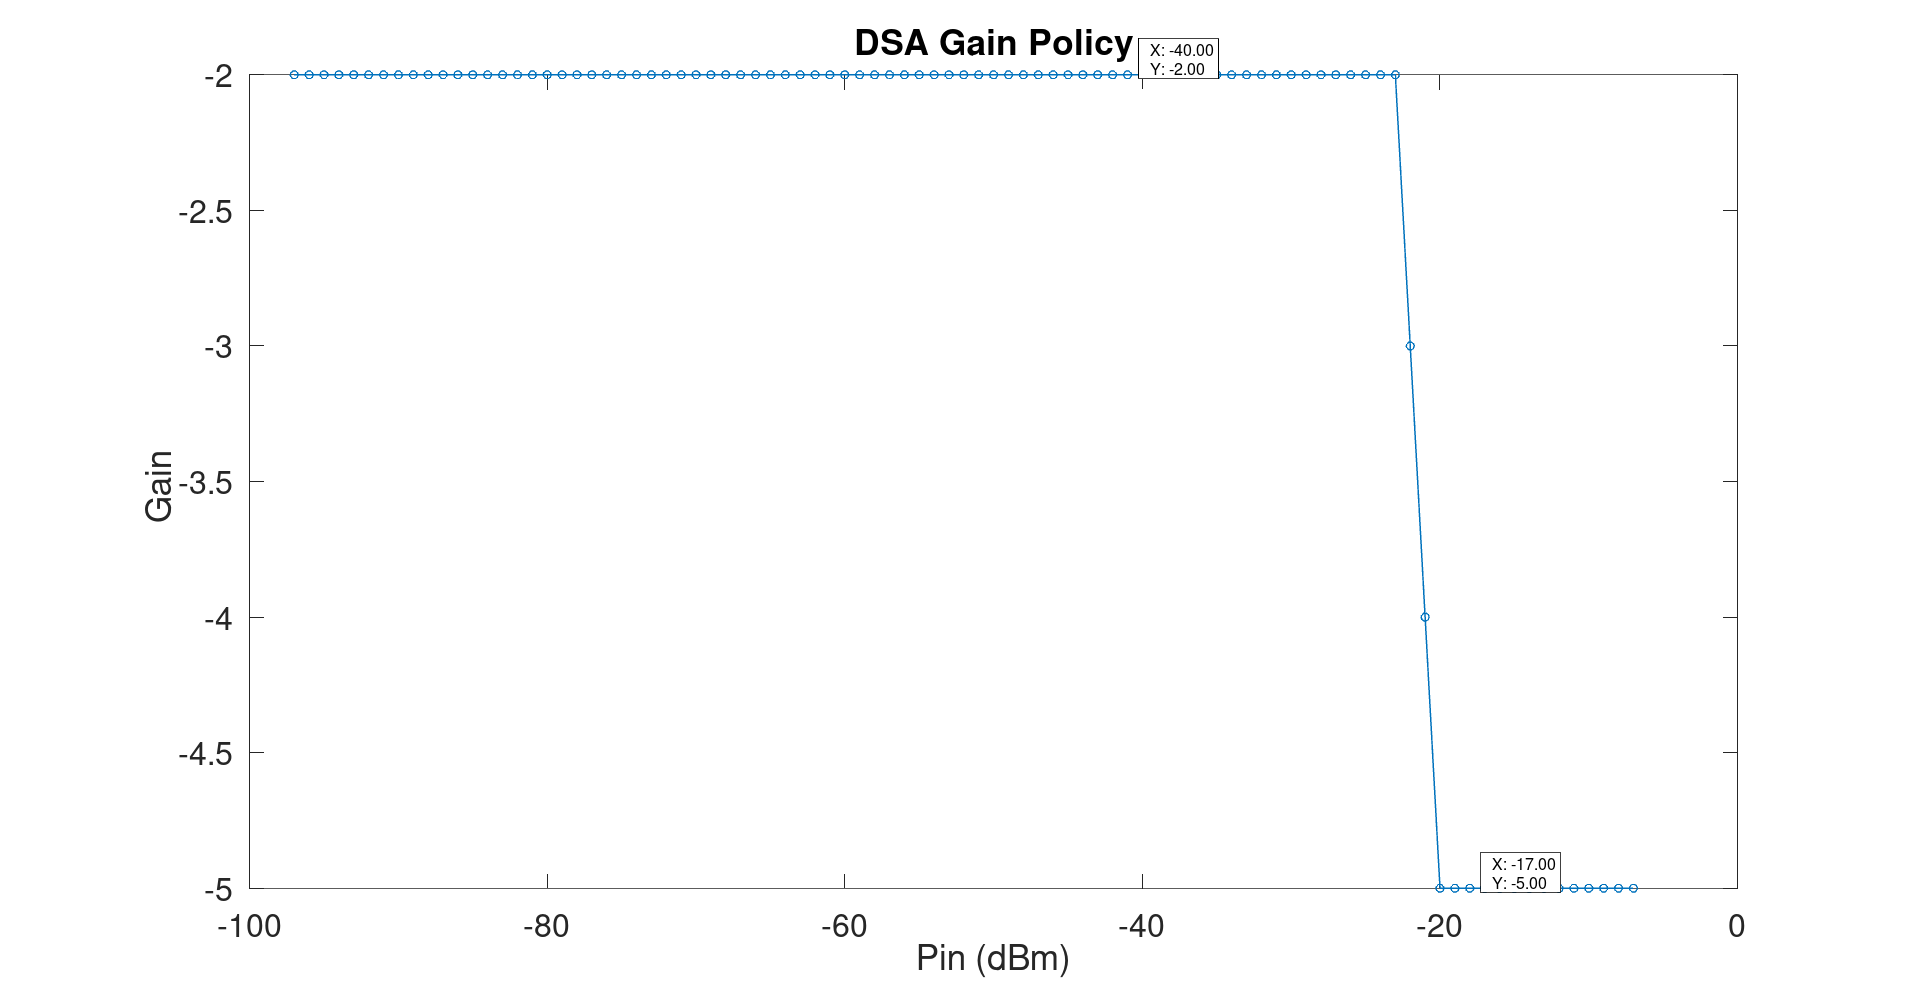
\includegraphics[width=1\linewidth]{images/DSA2_gain_policy_no_blockers.png}
  \caption{DSA 2 Gain Policy no blockers}
  \label{fig:DSA2_gain_policy_no_blockers.png}
\end{figure}


\begin{figure}[!h]
  \centering
  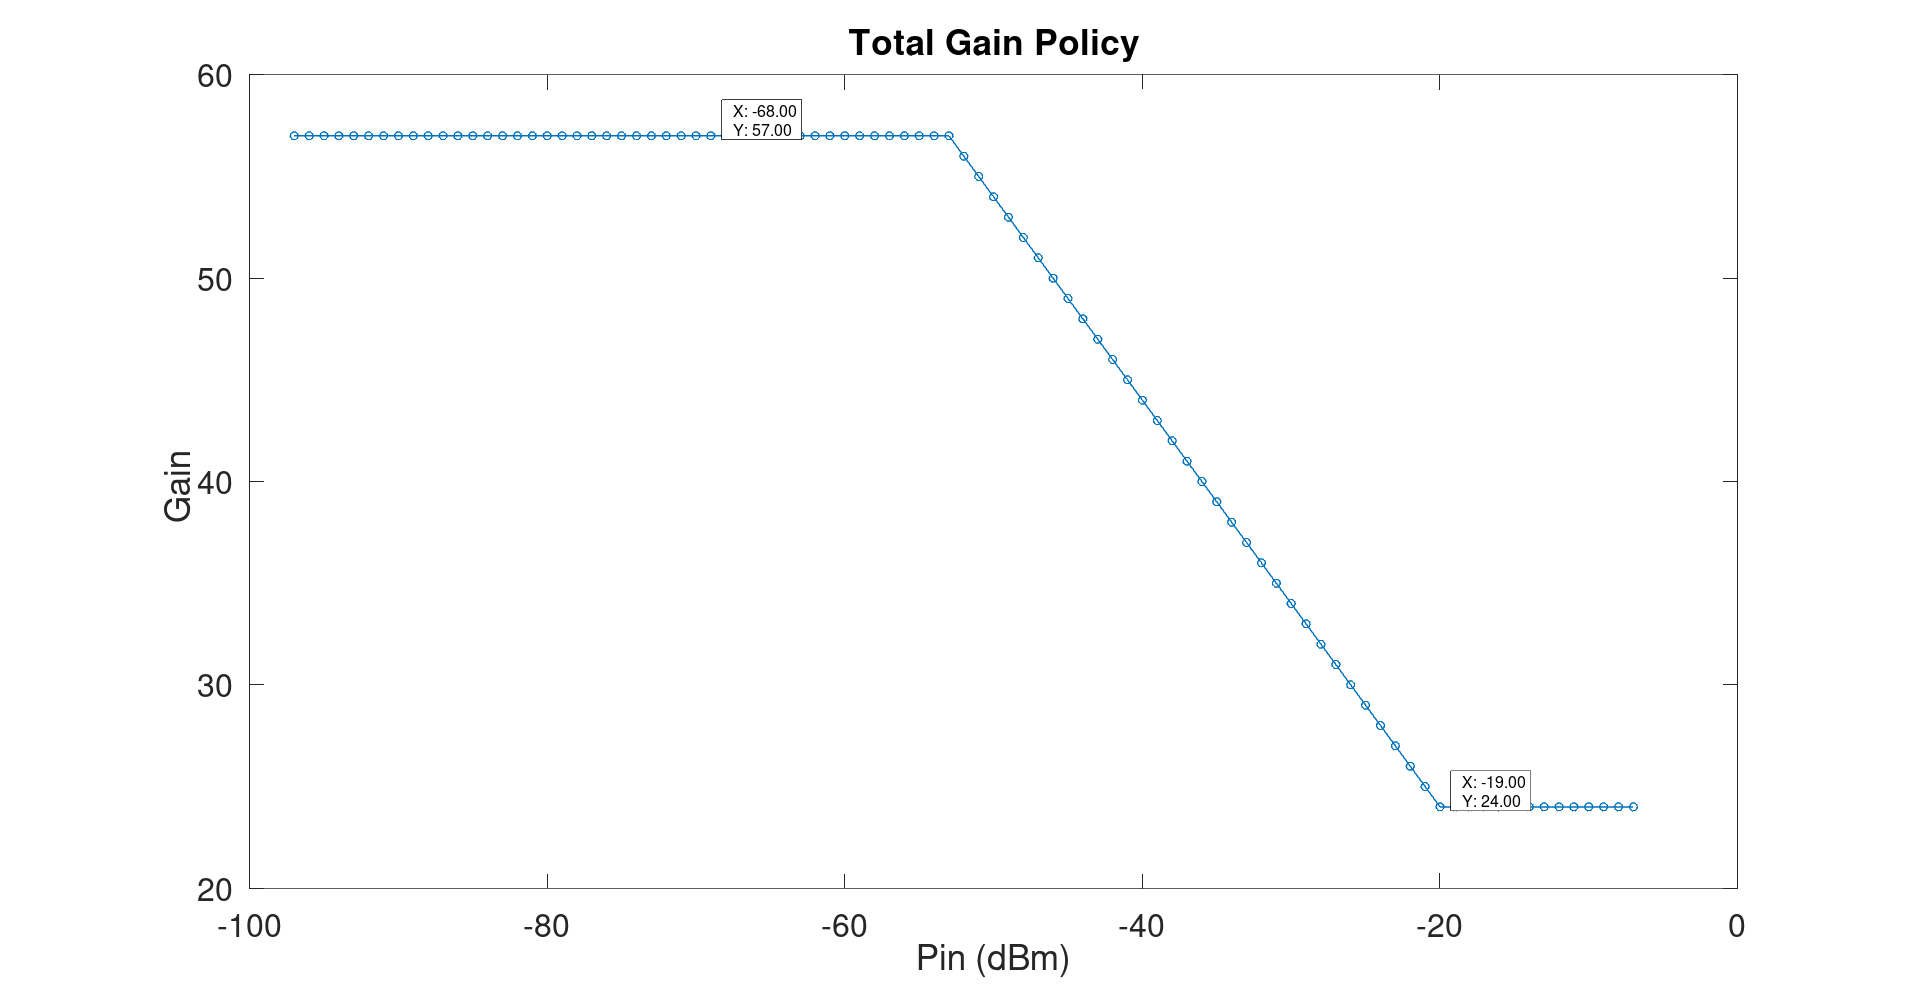
\includegraphics[width=1\linewidth]{images/total_gain_policy_no_blockers.png}
  \caption{Total Gain Policy no blockers}
  \label{fig:total_gain_policy_no_blockers.png}
\end{figure}
\clearpage

\subsubsection{Under blocking}%
\label{ssub:Under blocking}
Here results under blocking  , note that when the blocker exists DSA 1
attenuate 3dB inorder to overcome RF Amp compression (Figure~\ref{fig:DSA1_Gain_policy_under_blocking.png}),
Also DSA 1 starts the Attenuation because condition described by equation~\ref{eq:DSA_atten_cond} is satisfied.

\begin{figure}[!h]
  \centering
  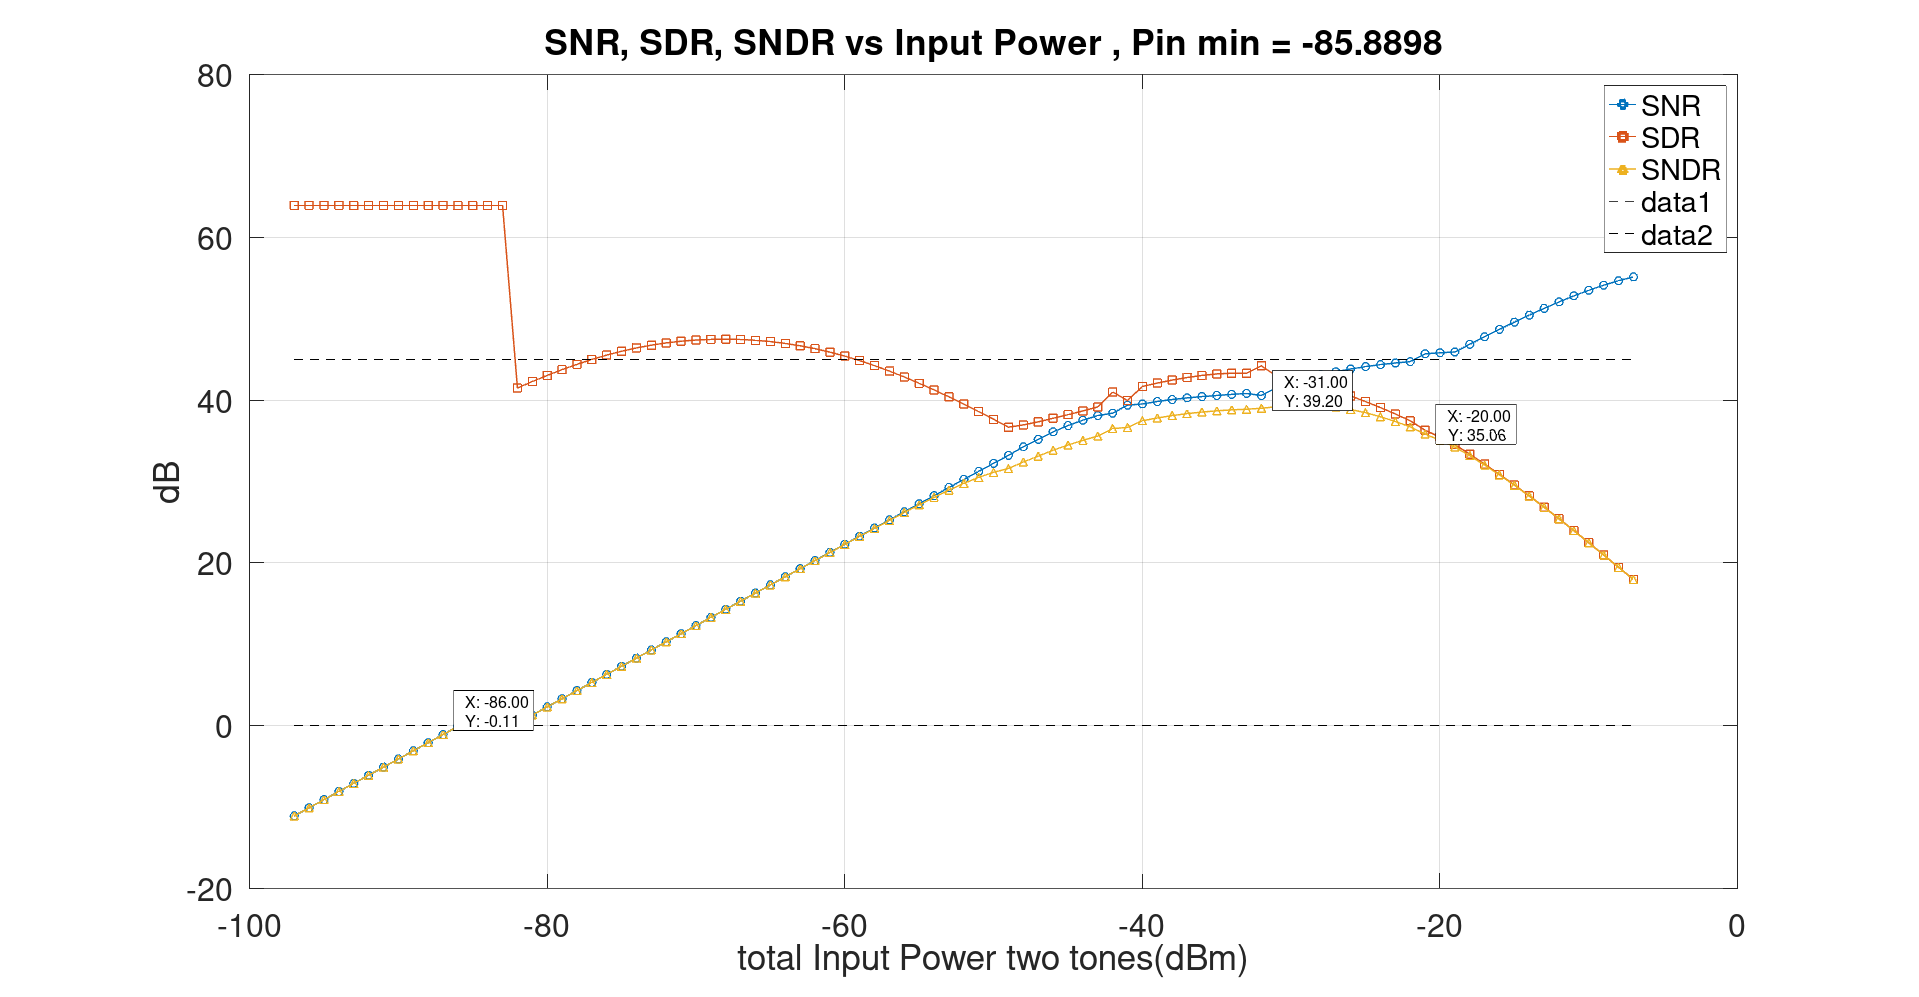
\includegraphics[width=1\linewidth]{images/SNDR_under_blocking.png}
  \caption{SNDR curve under blocking}
  \label{fig:SNDR_under_blocking.png}
\end{figure}

\begin{figure}[!h]
  \centering
  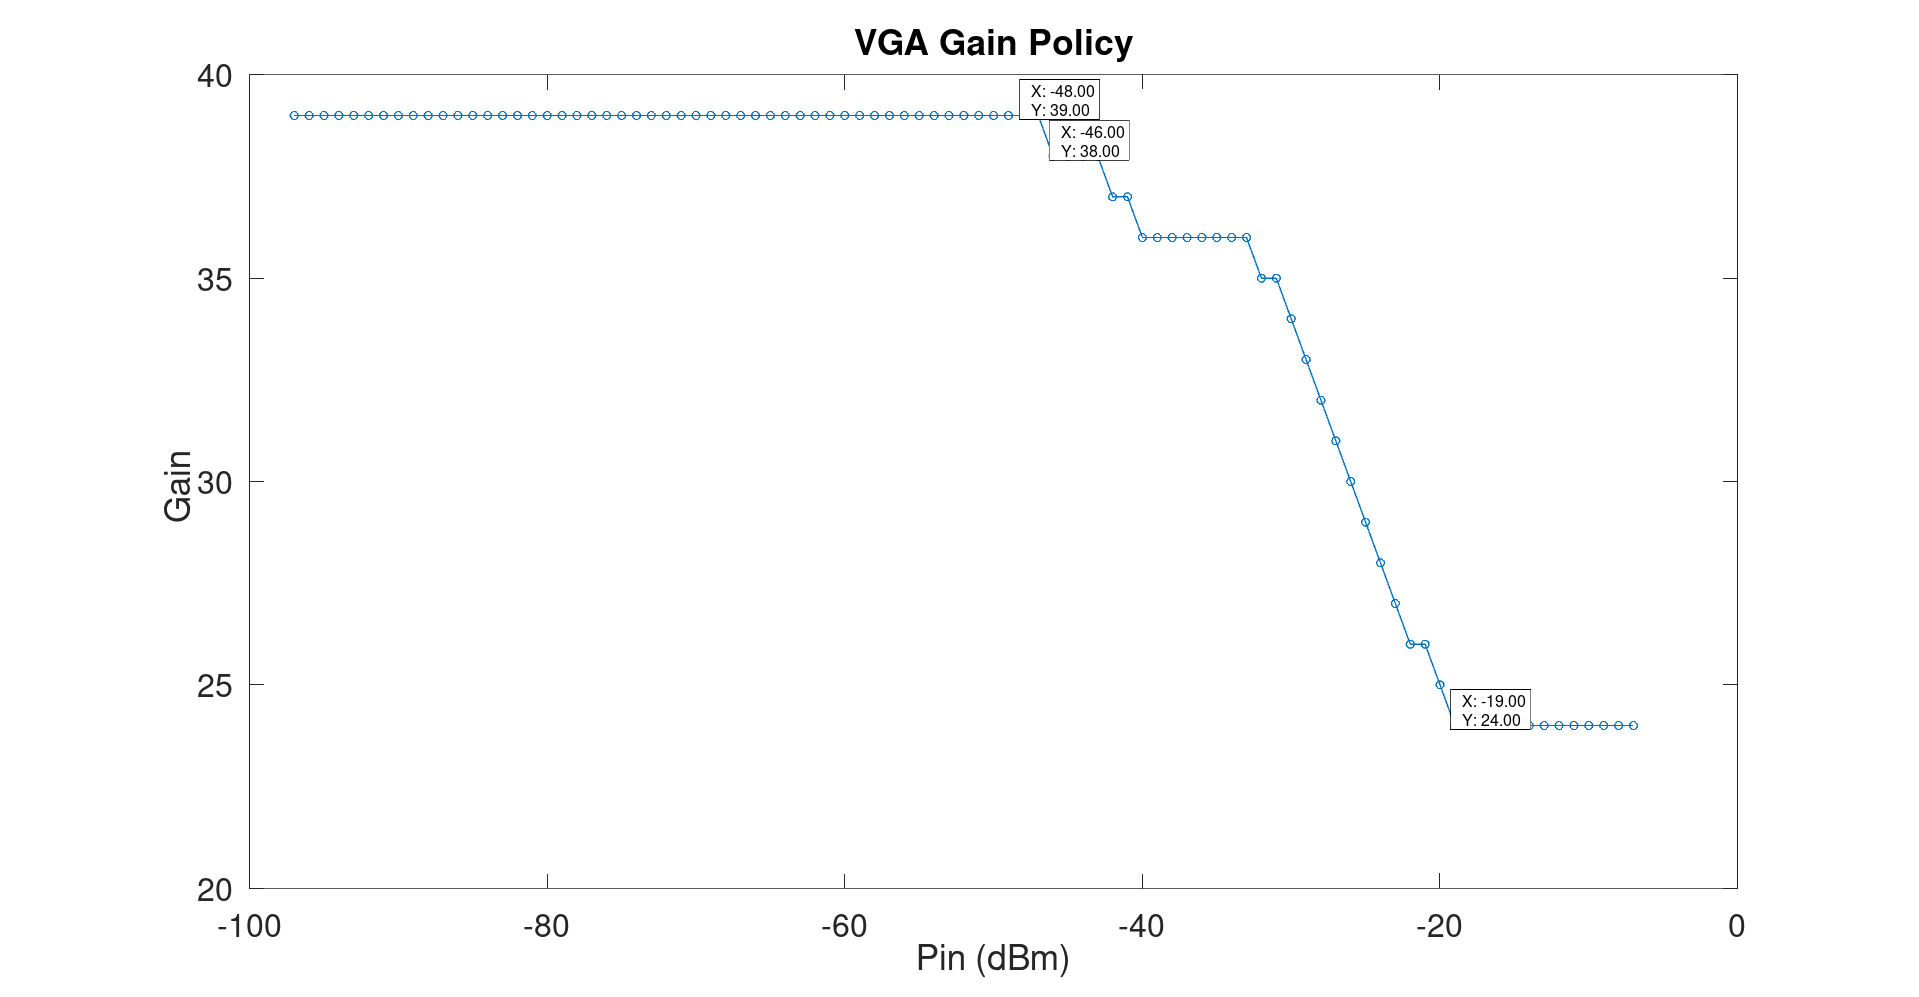
\includegraphics[width=1\linewidth]{images/VGA_policy_under_blocking.png}
  \caption{VGA gain Policy Under blocking}
  \label{fig:VGA_policy_under_blocking.png}
\end{figure}

\begin{figure}[!h]
  \centering
  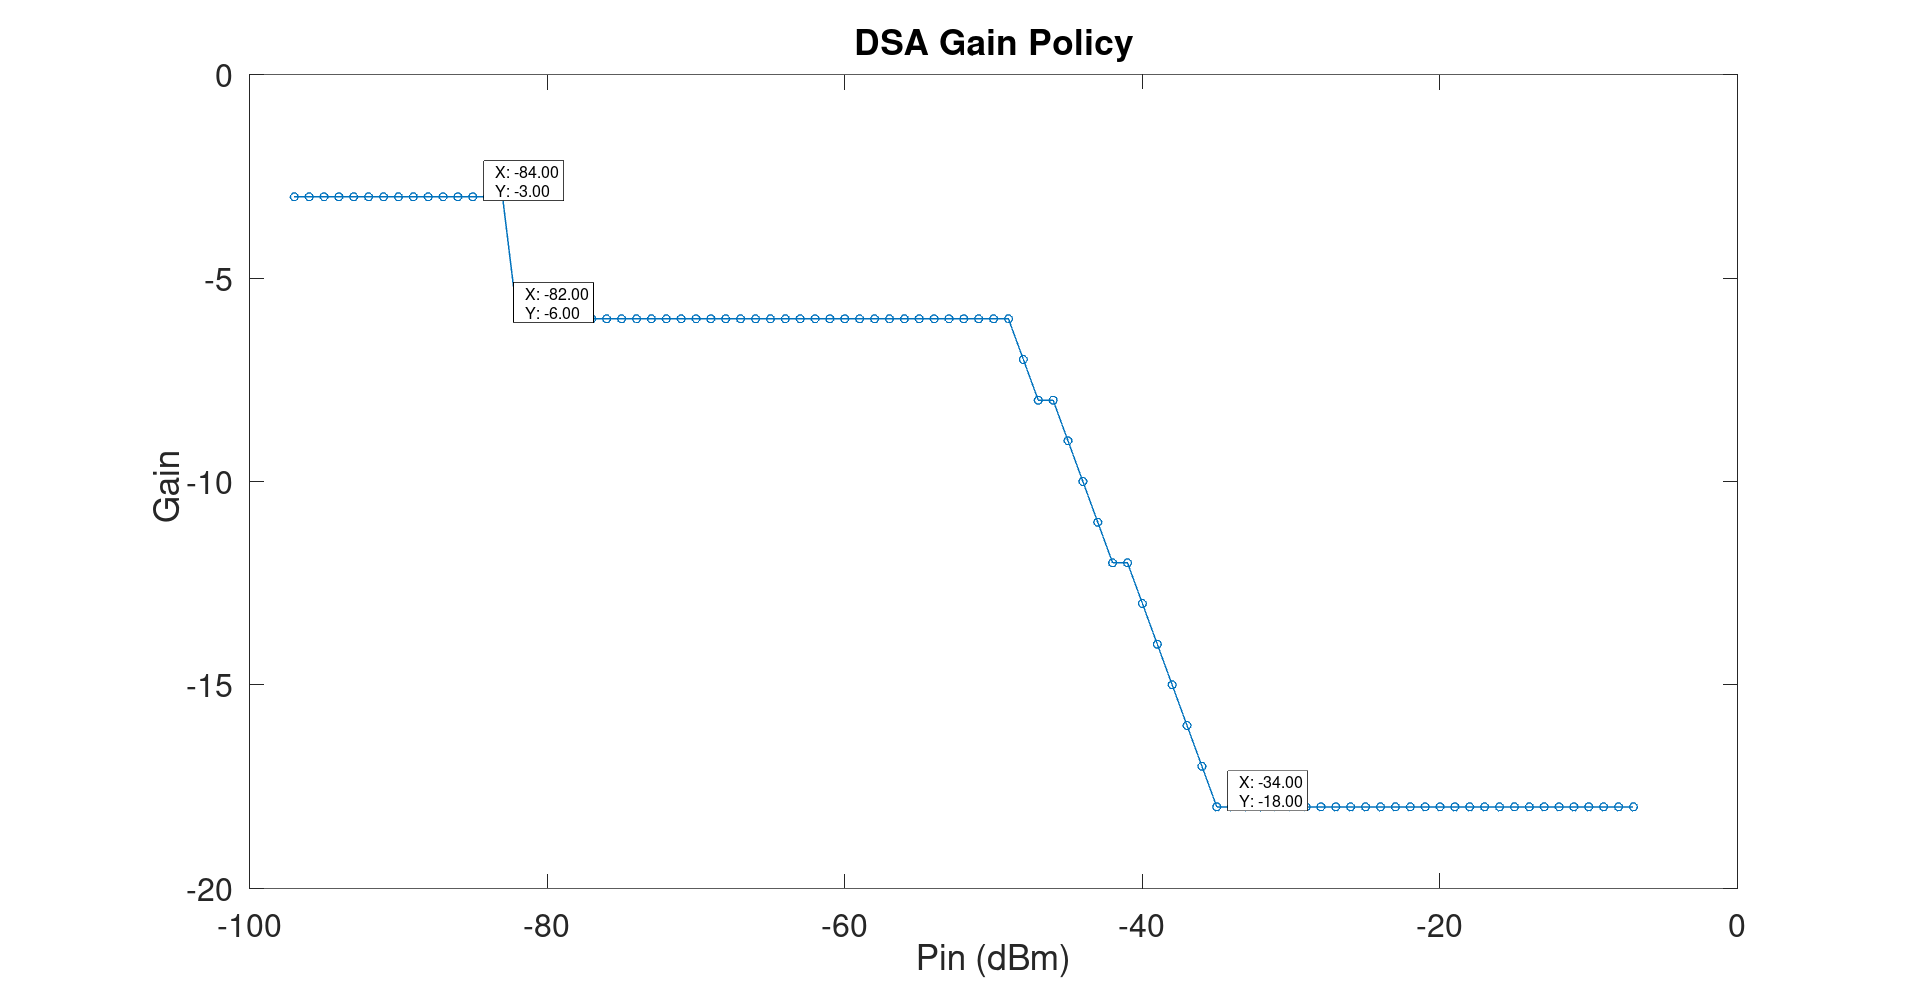
\includegraphics[width=1\linewidth]{images/DSA1_Gain_policy_under_blocking.png}
  \caption{DSA 1 gain policy under blocking}
  \label{fig:DSA1_Gain_policy_under_blocking.png}
\end{figure}

\begin{figure}[!h]
  \centering
  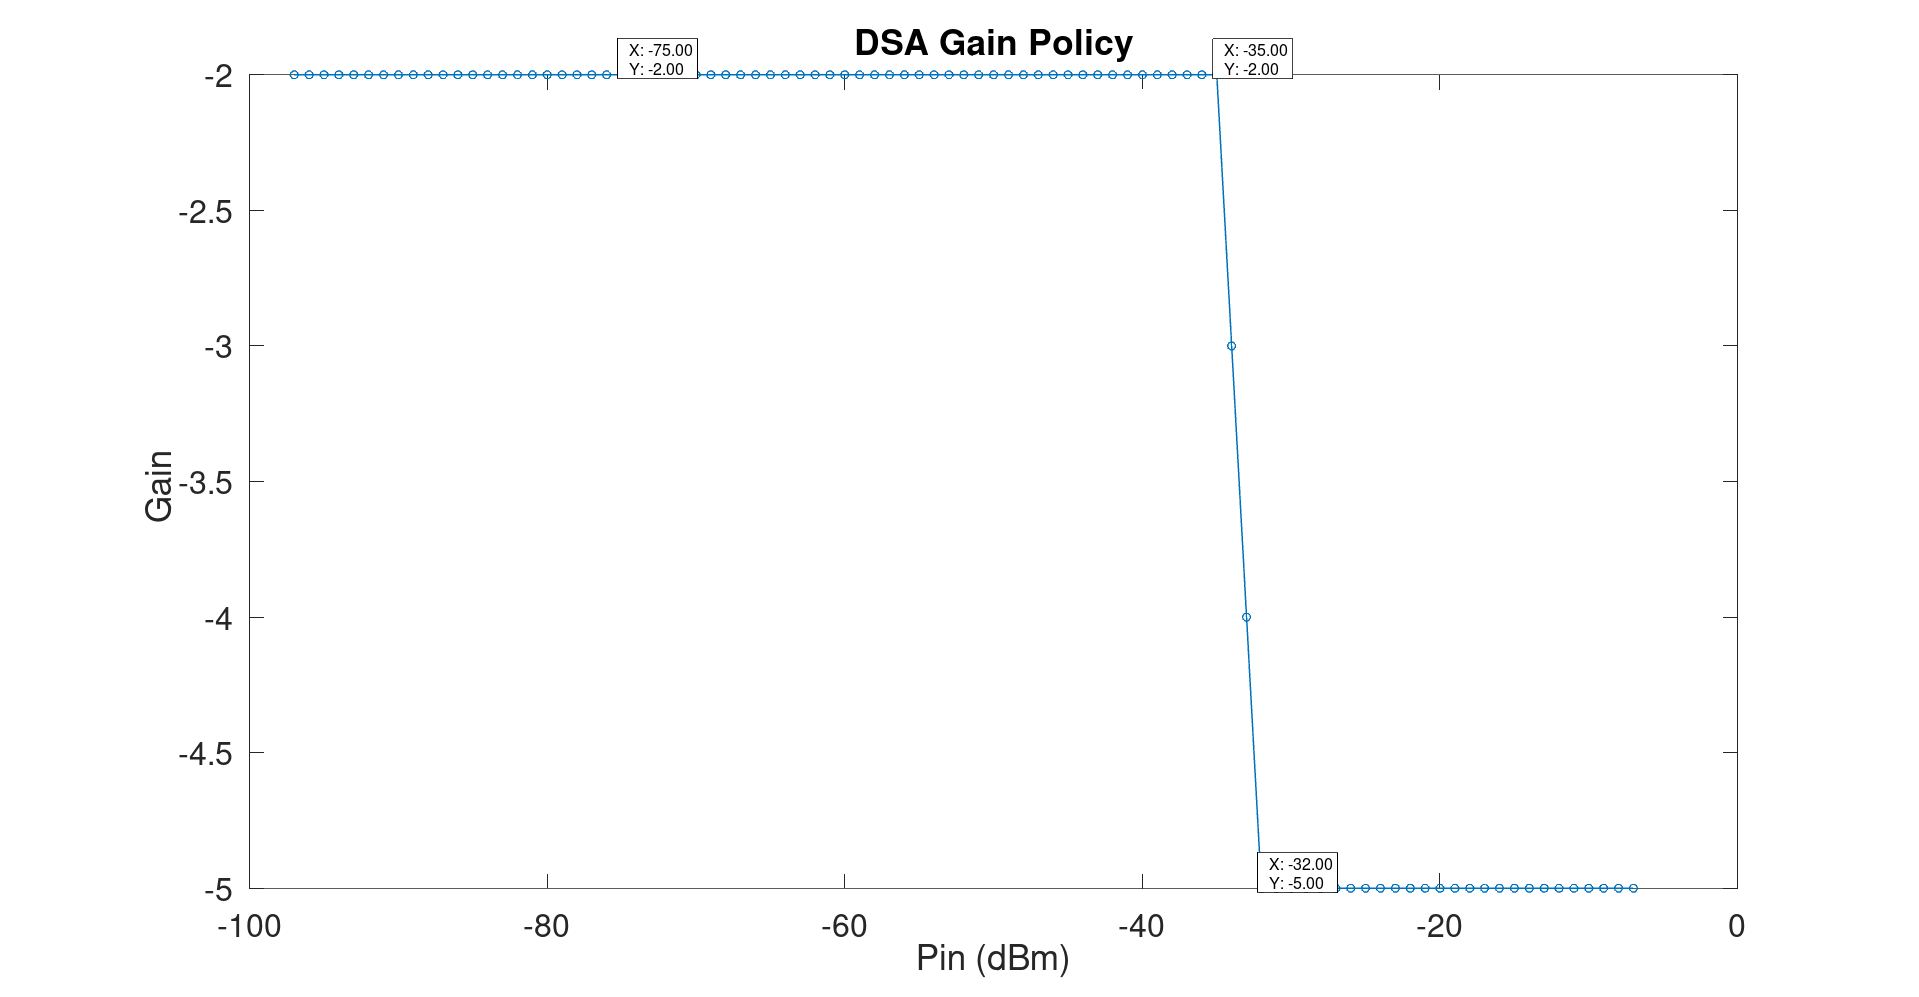
\includegraphics[width=1\linewidth]{images/DSA2_Gain_policy_under_blocking.png}
  \caption{DSA 2 Gain policy under blocking}
  \label{fig:DSA2_Gain_policy_under_blocking.png}
\end{figure}

\begin{figure}[!h]
  \centering
  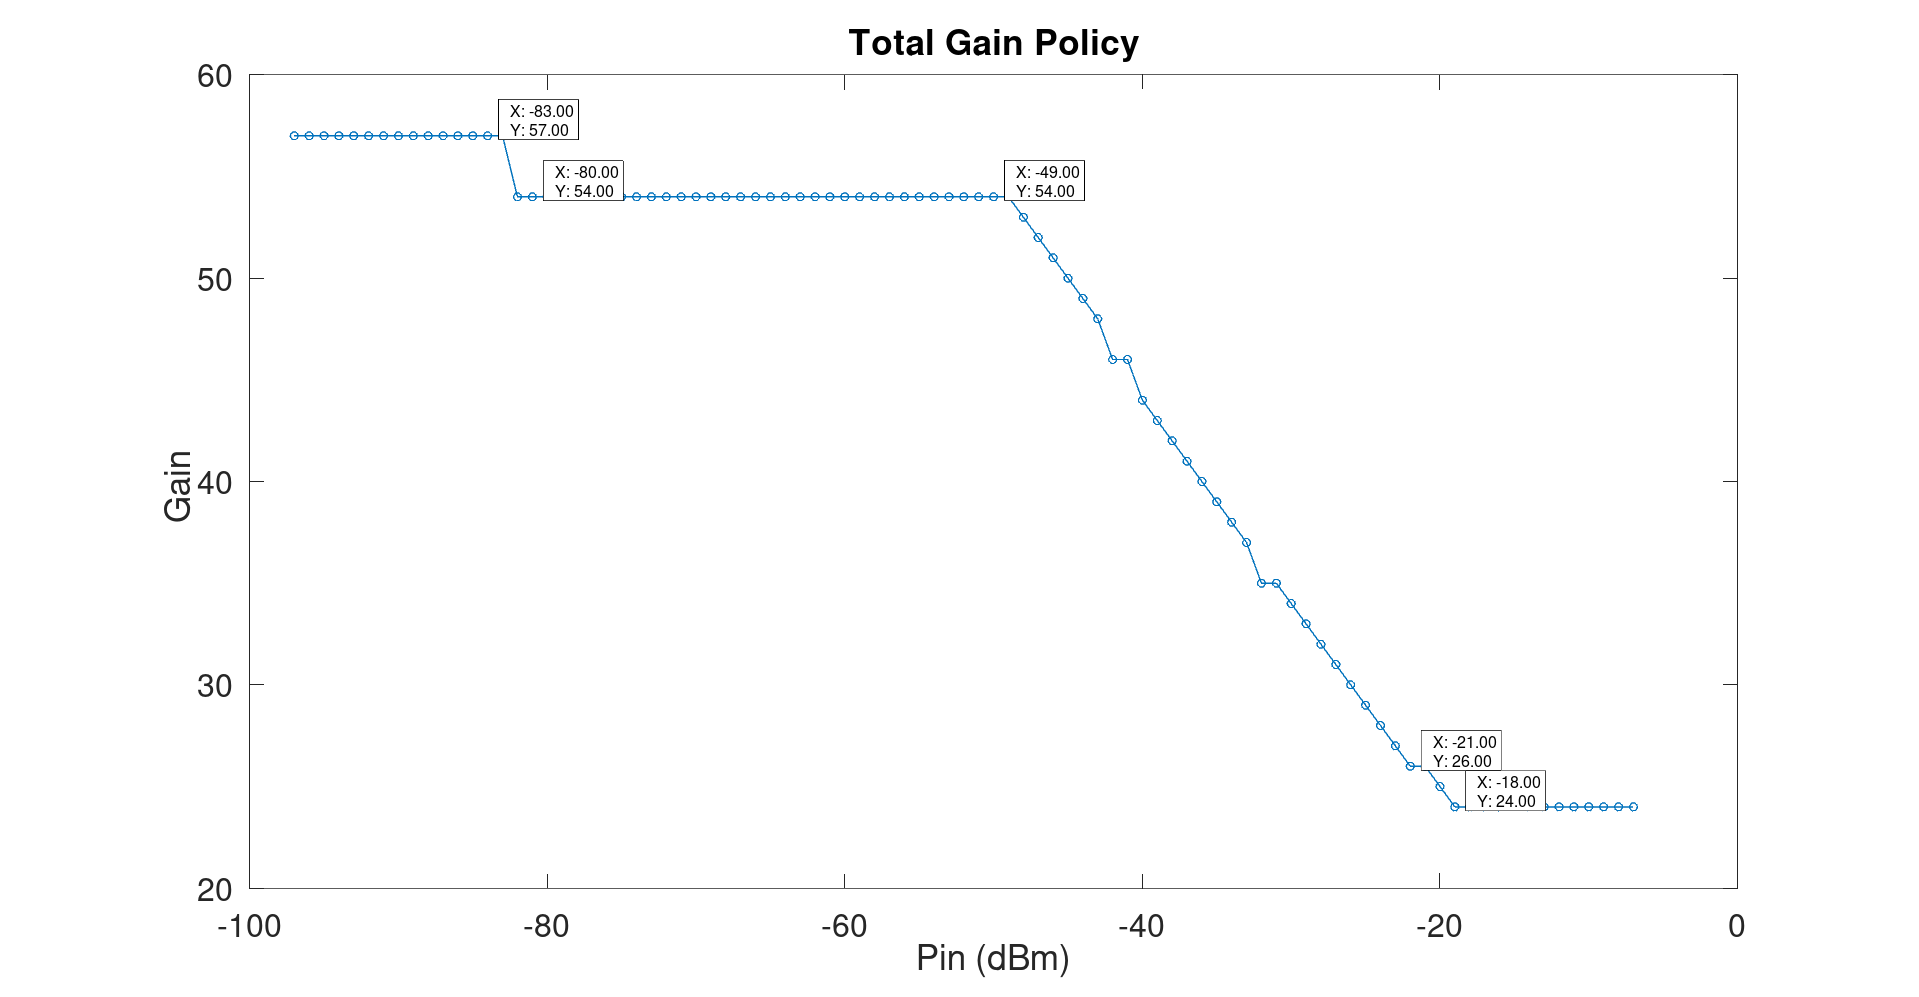
\includegraphics[width=1\linewidth]{images/Total_gain_policy_under_blocing.png}
  \caption{Total Gain policy Under blocking}
  \label{fig:Total_gain_policy_under_blocing.png}
\end{figure}











